\begin{center}
	\begin{tabular}{M{10cm}M{8cm}}
		\textbf{TRƯỜNG THCS-THPT NGUYỄN KHUYẾN}& \textbf{ÔN TẬP KTTX LẦN 2 HỌC KÌ I}\\
		\textbf{MÃ ĐỀ: 002}& \textbf{Bài thi môn: VẬT LÝ 10}\\
		\textit{(Đề thi có 05 trang)}& \textit{Thời gian: 40 phút, không kể phát đề}
		
		\noindent\rule{4cm}{0.8pt} \\
	\end{tabular}
\end{center}
\setcounter{section}{0}
\section{Câu trắc nghiệm nhiều phương án lựa chọn}
\textit{Thí sinh trả lời từ câu 1 đến câu 20. Mỗi câu hỏi thí sinh chọn một phương án}
\setcounter{ex}{0}
\Opensolutionfile{ans}[ans/D10-HKI-KTTX2-002-TN]
% ===================================================================
\begin{ex}
	Hệ thức nào sau đây là đúng theo định luật II Newton?
	\choice
	{\True $\vec{F}=m\vec{a}$}
	{$a=\dfrac{F}{m}$}
	{$\vec{a}=\dfrac{F}{m}$}
	{$\vec{F}=-m\vec{a}$}
	\loigiai{}
\end{ex}
% ===================================================================
\begin{ex}
	Khối lượng là đại lượng đặc trưng cho
	\choice
	{trọng lượng của vật}
	{tác dụng làm quay của lực quanh một trục}
	{thể tích của vật}
	{\True mức quán tính của vật}
	\loigiai{}
\end{ex}
% ===================================================================
\begin{ex}
	Một chất điểm chịu tác dụng đồng thời của hai lực $\vec{F}_1$ và $\vec{F}_2$ thì hợp lực $\vec{F}$ của chúng luôn có độ lớn thỏa mãn hệ thức	
	\choice
	{$F=F_1-F_2$}
	{$F=F_1+F_2$}
	{\True $\left|F_1-F_2\right|\le F\le F_1+F_2$}
	{$F^2=F^2_1+F^2_2$}
	\loigiai{}
\end{ex}
% ===================================================================
\begin{ex}
	Một vật đang chuyển động nhanh dần đều dưới tác dụng của lực kéo mà lực đó đột ngột giảm độ lớn thì
	\choice
	{gia tốc của vật không đổi}
	{\True gia tốc của vật giảm}
	{gia tốc của vật tăng}
	{gia tốc và vận tốc của vật đều giảm}
	\loigiai{}
\end{ex}
% ===================================================================
\begin{ex}
	Khi đang đi xe đạp trên đường nằm ngang, nếu ta ngừng đạp, xe vẫn còn đi tiếp chưa dừng lại ngay là nhờ
	\choice
	{trọng lượng của xe}
	{lực ma sát}
	{\True quán tính của xe}
	{phản lực của mặt đường}
	\loigiai{}
\end{ex}
% ===================================================================
\begin{ex}
	Theo định luật I Newton thì 	
	\choice
	{lực là nguyên nhân duy trì chuyển động}
	{\True một vật sẽ giữ nguyên trạng thái đứng yên hoặc chuyển động thẳng đều nếu nó không chịu tác dụng của lực nào}
	{một vật không thể chuyển động được nếu hợp lực tác dụng lên nó bằng 0}
	{mọi vật đang chuyển động đều có xu hướng dừng lại do quán tính}
	\loigiai{}
\end{ex}
% ===================================================================
\begin{ex}
	Một xe ô tô đang chuyển động thẳng với vận tốc không đổi là $\SI{20}{\meter/\second}$. Hợp lực tác dụng lên ô tô có độ lớn bằng
	\choice
	{$\SI{20}{\newton}$}
	{\True $0$}
	{$\SI{10}{\newton}$}
	{$\SI{-20}{\newton}$}
	\loigiai{}
\end{ex}
% ===================================================================
\begin{ex}
	Khi một ô tô đột ngột phanh gấp thì người ngồi trong xe	
	\choice
	{ngả người về sau}
	{\True chúi người về phía trước}
	{ngả người sang bên cạnh}
	{dừng lại ngay}
	\loigiai{}
\end{ex}
% ===================================================================
\begin{ex}
	Những nhận định nào sau đây là đúng?
	\begin{enumerate}[label=\arabic*.]
		\item Khi vật chịu tác dụng của lực $\vec{F}$ thì gia tốc $\vec{a}$ mà vật thu được cùng phương nhưng ngược chiều với $\vec{F}$.
		\item Khi vật chỉ chịu tác dụng của lực $\vec{F}$ thì gia tốc $\vec{a}$ mà vật thu được cùng hướng với $\vec{F}$.
		\item Khi vật chịu tác dụng của hai lực cân bằng thì gia tốc $\vec{a}$ của vật thu được khác không.
		\item Khi vật chịu tác dụng của nhiều lực thì gia tốc $\vec{a}$ của vật thu được cùng hướng với lực tổng hợp tác dụng lên vật.
	\end{enumerate}
	\choice
	{\True 2, 4}
	{1, 3}
	{1, 4}
	{3, 4}
	\loigiai{}
\end{ex}
% ===================================================================
\begin{ex}
	Một lực $F_1$ không đổi, tác dụng lên vật khối lượng $m_1$ làm cho vật thu được gia tốc $a_1$.  Một lực $F_2$ không đổi, tác dụng lên vật khối lượng $m_2$ làm cho vật thu được gia tốc $a_2$. Nếu $F_2=F_1/3$ và $m_1=2m_2/5$ thì tỉ số $a_1/a_2$ bằng
	\choice
	{\True 15/2}
	{6/5}
	{11/15}
	{5/6}
	\loigiai{}
\end{ex}
% ===================================================================
\begin{ex}
	Tác dụng vào vật có khối lượng $\SI{3}{\kilogram}$ đang đứng yên một lực theo phương ngang thì vật này chuyển động nhanh dần đều với gia tốc $\SI{1.5}{\meter/\second^2}$. Độ lớn của lực này là
	\choice
	{$\SI{3}{\newton}$}
	{\True $\SI{4.5}{\newton}$}
	{$\SI{1.5}{\newton}$}
	{$\SI{2}{\newton}$}
	\loigiai{}
\end{ex}
% ===================================================================
\begin{ex}
	Một mẫu siêu xe có khối lượng $\SI{1.60}{\text{tấn}}$. Nếu coi xe tăng tốc đều và lực trung bình để tăng tốc xe là $\SI{24.0}{\kilo\newton}$ thì mẫu xe này cần bao lâu để có thể tăng tốc từ trạng thái nghỉ lên đến tốc độ $\SI{108}{\kilo\meter/\hour}$?
	\choice
	{\True Khoảng $\SI{2.00}{\second}$}
	{Khoảng $\SI{7.20}{\second}$}
	{Khoảng $\SI{10.0}{\second}$}
	{Khoảng $\SI{15.0}{\second}$}
	\loigiai{}
\end{ex}
% ===================================================================
\begin{ex}
	Một vật có khối lượng $m=\SI{10}{\kilogram}$ đang chuyển động thẳng đều với tốc độ $v=\SI{10}{\meter/\second}$ thì chịu tác dụng của một lực $\vec{F}$ không đổi, ngược hướng chuyển động và có độ lớn $F=\SI{10}{\newton}$.\\ Nhận định nào sau đây về chuyển động của vật là đúng?
	\choice
	{Vật dừng lại ngay}
	{\True Sau $\SI{10}{\second}$ kể từ lúc lực $\vec{F}$ tác dụng thì vật sẽ chuyển động theo chiều ngược lại}
	{Vật chuyển động chậm dần rồi dừng lại}
	{}
	\loigiai{}
\end{ex}
% ===================================================================
\begin{ex}
	Chất điểm khối lượng $\SI{2}{\kilogram}$ đứng yên dưới tác dụng của ba lực đồng qui có độ lớn lần lượt là $\SI{10}{\newton}$, $\SI{20}{\newton}$, $\SI{30}{\newton}$. Nếu bỏ đi lực $\SI{20}{\newton}$ thì
	\choice
	{chất điểm chuyển động thẳng đều}
	{chất điểm tiếp tục đứng yên}
	{\True chất điểm chuyển nhanh dần đều với gia tốc có độ lớn $\SI{10}{\meter/\second^2}$}
	{chất điểm chuyển nhanh dần đều với gia tốc có độ lớn $\SI{5}{\meter/\second^2}$}
	\loigiai{}
\end{ex}
% ===================================================================
\begin{ex}
	Một lực không đổi tác dụng vào một vật có khối lượng $\SI{7.5}{\kilogram}$ làm vật thay đổi tốc độ từ $\SI{8}{\meter/\second}$ đến $\SI{3}{\meter/\second}$ trong khoảng thời gian $\SI{2}{\second}$ nhưng vẫn giữ nguyên chiều chuyển động. Lực tác dụng vào vật có giá trị là
	\choice
	{$\SI{18.75}{\newton}$}
	{\True $\SI{-18.75}{\newton}$}
	{$\SI{20.5}{\newton}$}
	{$\SI{-20.5}{\newton}$}
	\loigiai{}
\end{ex}
% ===================================================================
\begin{ex}
	Một chất điểm chịu tác dụng của hai lực có độ lớn $\SI{18}{\newton}$ và $\SI{24}{\newton}$. Biết hợp lực của hai lực này có giá trị $\SI{30}{\newton}$, góc tạo bởi hai lực này là
	\choice
	{\True $\SI{90}{\degree}$}
	{$\SI{30}{\degree}$}
	{$\SI{45}{\degree}$}
	{$\SI{60}{\degree}$}
	\loigiai{}
\end{ex}
% ===================================================================
\begin{ex}
	Một xe tải chở hàng có tổng khối lượng xe và hàng hóa là 4 tấn, khởi hành với gia tốc $\SI{0.3}{\meter/\second^2}$. Khi không chở hàng, xe tải khởi hành với tốc $\SI{0.6}{\meter/\second^2}$. Biết rằng hợp lực tác dụng vào ô tô trong hai trường hợp đều bằng nhau. Khối lượng của xe lúc không chở hàng là
	\choice
	{1 tấn}
	{1,5 tấn}
	{\True 2 tấn}
	{2,5 tấn}
	\loigiai{}
\end{ex}
% ===================================================================
\begin{ex}
	Một xe tải không chở hàng đang chạy trên đường. Nếu người lái xe hãm phanh thì xe trượt một đoạn đường $\SI{12}{\meter}$ thì dừng lại. Nếu xe chở hàng có khối lượng hàng bằng hai lần khối lượng xe thì đoạn đường trượt bằng bao nhiêu? Cho rằng lực hãm và vận tốc ban đầu của xe tải không đổi.
	\choice
	{$\SI{4}{\meter}$}
	{$\SI{6}{\meter}$}
	{$\SI{24}{\meter}$}
	{\True $\SI{36}{\meter}$}
	\loigiai{}
\end{ex}
% ===================================================================
\begin{ex}
	Một vật nhỏ có khối lượng $\SI{10}{\kilogram}$ đang chuyển động với tốc độ $\SI{3}{\meter/\second}$ thì chịu tác động của một lực $\vec{F}$ cùng phương, cùng chiều chuyển động. Khi đó vật chuyển động nhanh dần đều và sau khi đi được thêm $\SI{32}{\meter}$ thì có tốc độ $\SI{5}{\meter/\second}$. Lực tác dụng vào vật có độ lớn bằng
	\choice
	{$\SI{0.25}{\newton}$}
	{\True $\SI{2.5}{\newton}$}
	{$\SI{25}{\newton}$}
	{$\SI{16}{\newton}$}
	\loigiai{}
\end{ex}
% ===================================================================
\begin{ex}
	Một lực tác dụng vào vật trong khoảng thời gian $\SI{0.6}{\second}$ làm vận tốc của nó thay đổi từ $\SI{8}{\centi\meter/\second}$ đến $\SI{5}{\centi\meter/\second}$ (lực cùng phương với phương chuyển động). Tiếp đó, tăng độ lớn của lực lên gấp đôi trong khoảng thời gian $\SI{2.2}{\second}$ nhưng vẫn giữ nguyên hướng của lực. Vận tốc của vật tại thời điểm cuối là
	\choice
	{$\SI{12}{\centi\meter/\second}$}
	{$\SI{15}{\centi\meter/\second}$}
	{\True $\SI{-17}{\centi\meter/\second}$}
	{$\SI{-20}{\centi\meter/\second}$}
	\loigiai{}
\end{ex}
\Closesolutionfile{ans}
\section{Câu trắc nghiệm đúng/sai} 
\textit{Thí sinh trả lời từ câu 1 đến câu 2. Trong mỗi ý \textbf{a)}, \textbf{b)}, \textbf{c)}, \textbf{d)} ở mỗi câu, thí sinh chọn đúng hoặc sai}
\setcounter{ex}{0}\\
\Opensolutionfile{ans}[ans/D10-HKI-KTTX2-002-TF]
% ===================================================================
\begin{ex}
	Một cậu bé đứng trên thùng xe của một chiếc xe bán tải đang chuyển động thẳng đều trên một đoạn đường nằm ngang. Cậu bé ném một lon nước ngọt theo phương thẳng đứng lên cao như hình minh họa bên dưới.
	\begin{center}
		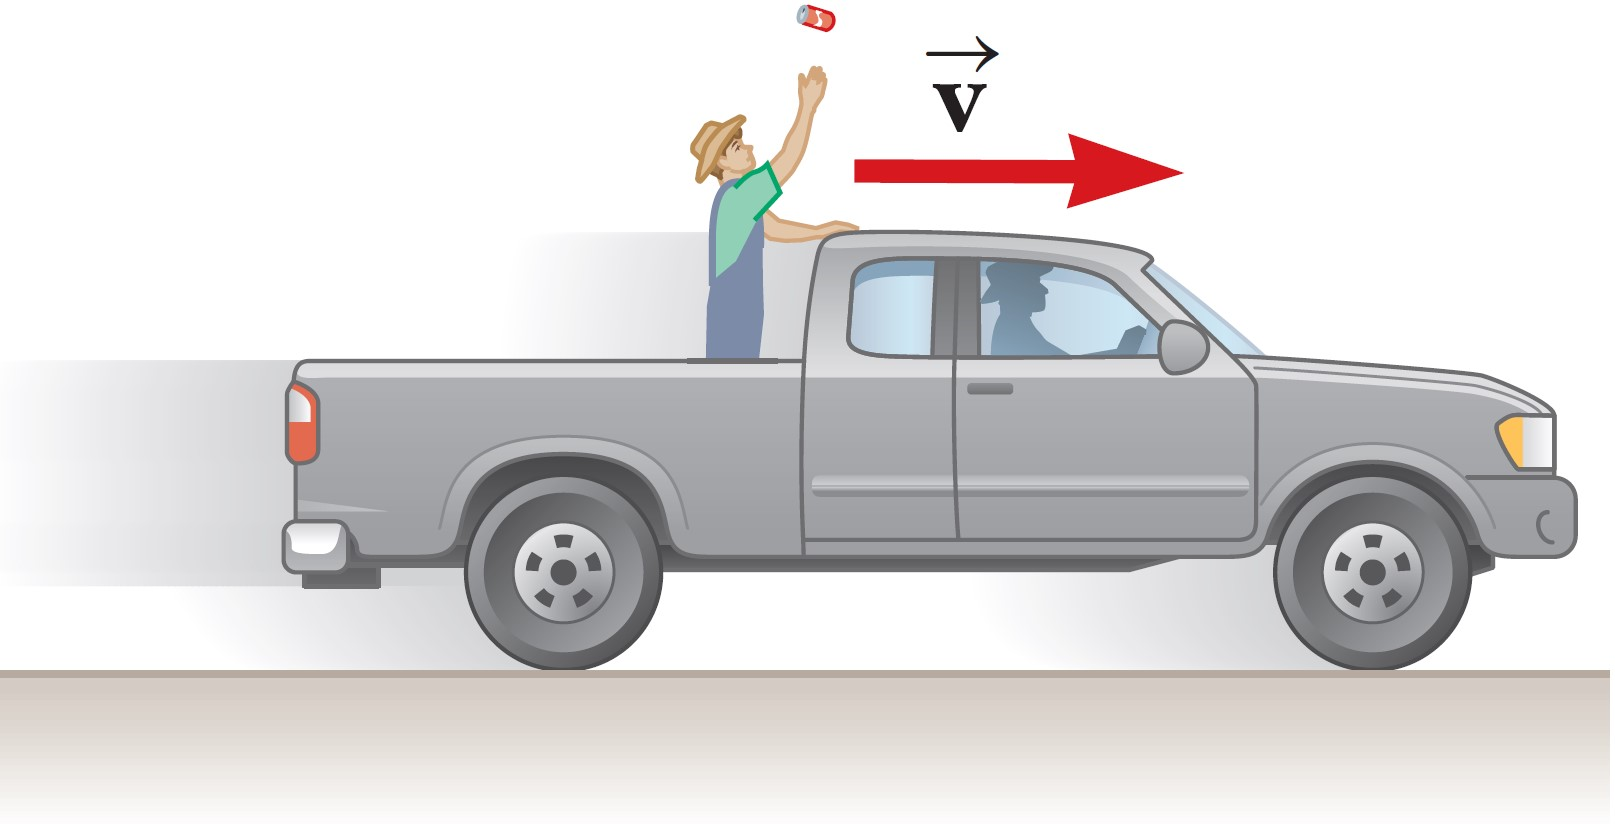
\includegraphics[width=0.4\linewidth]{figs/D10-HKI-KTTX2-001-4}
	\end{center}
	\choiceTF[t]
	{\True Lon nước ngọt sẽ rơi trở lại về tay cậu bé}
	{Đối với người quan sát đang đứng yên bên đường, lon nước ngọt chuyển động theo phương thẳng đứng}
	{\True Nếu xe tăng tốc trong quá trình lon nước rơi, lon nước sẽ rơi về phía sau cậu bé}
	{\True Nếu xe giảm tốc trong quá trình lon nước rơi, lon nước sẽ rơi về phía trước cậu bé}
	\loigiai{}
\end{ex}
% ===================================================================
\begin{ex}
	Hai thanh dầm thép đồng chất, có trọng tâm (điểm đặt của trọng lực) tại A và B, đặt chồng lên nhau như hình bên. Thanh dài hơn có trọng lượng $\SI{10}{\kilo\newton}$.
	\begin{center}
		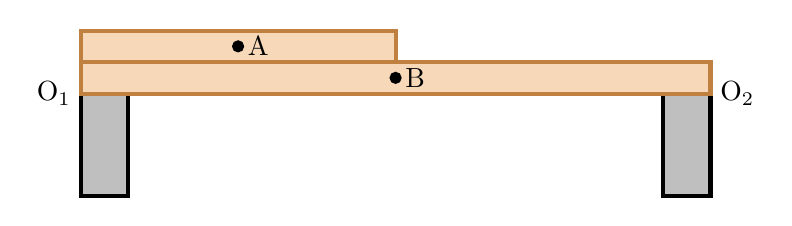
\begin{tikzpicture}
			\filldraw[line width=1.5pt, black, fill=gray!50!white] (0,-0.2) rectangle (0.6,-1.5);
			\filldraw[line width=1.5pt, black, fill=gray!50!white] (7.4,-0.2) rectangle (8,-1.5);
			\filldraw[line width=1.5pt, brown, fill=orange!60!brown!30!white] (0,-0.2) rectangle (8,0.2);
			\filldraw[line width=1.5pt, brown, fill=orange!60!brown!30!white] (0,0.2) rectangle (4,0.6);
			\filldraw (4,0) circle(2pt) node[right] {B};
			\filldraw (2,0.4) circle(2pt) node[right] {A};
			\node[left] at (0,-0.2) {O$_1$};
			\node[right] at (8,-0.2) {O$_2$};
		\end{tikzpicture}
	\end{center}
	Hai thanh dầm được đặt lên các cột đỡ tại $O_1$ và $O_2$. Hệ ở trạng thái cân bằng.
	\choiceTF[t]
	{\True Trọng lượng của thanh dầm ngắn hơn là $\SI{5}{\kilo\newton}$}
	{Hợp lực $\vec{P}$ của các trọng lực tác dụng lên hai thanh dầm có độ lớn $\SI{12.5}{\kilo\newton}$}
	{Khoảng cách từ giá của hợp lực $\vec{P}$ đến cột $O_1$ gấp 1,4 lần khoảng cách đến cột O$_2$}
	{\True Lực nâng của cột đỡ O$_1$ tác dụng lên thanh dầm có độ lớn $\SI{8.75}{\newton}$}
	\loigiai{}
\end{ex}
\Closesolutionfile{ans}
\section{Câu trắc nghiệm trả lời ngắn} \textit{Thí sinh trả lời từ câu 1 đến câu 6}
\setcounter{ex}{0}
\Opensolutionfile{ans}[ans/D10-HKI-KTTX2-002-TL]
% ===============================================================
\begin{ex}
	Một ô tô có các thông số gồm:
	\begin{center}
		\begin{tabular}{|M{5cm}|M{5cm}|M{5cm}|}
			\hline
			\thead{Khối lượng $\left(\si{\kilogram}\right)$} &\thead{Tải trọng $\left(\si{\kilogram}\right)$}&\thead{Tốc độ tối ưu $\left(\si{\kilo\meter/\hour}\right)$}\\
			\hline
			$\SI{2.10E3}{}$ & $950$ & $75,6$\\
			\hline
		\end{tabular}
	\end{center}
	Khi ô tô chở đủ tải trọng, nó có thể tăng tốc từ trạng thái nghỉ đến tốc độ tối ưu trong $\SI{3.00}{\text{giây}}$. Độ lớn lực tác dụng lên ô tô khi tăng tốc là bao nhiêu kilo newton $\left(\si{\kilo\newton}\right)$? \textit{(Làm tròn kết quả đến chữ số hàng phần mười)}.
	\shortans[oly]{21,4}
	\loigiai{
		
	}
\end{ex}
% ===============================================================
\begin{ex}
	Một quả bóng tennis khối lượng $\SI{56}{\gram}$ đang bay với tốc độ $\SI{20}{\meter/\second}$ thì đập trực diện vào bức tường và bật ngược trở lại với tốc độ $\SI{15}{\meter/\second}$. Thời gian quả bóng va chạm với tường là $\SI{0.05}{\second}$. Chọn chiều dương là chiều chuyển động ban đầu của quả bóng. Xác định lực do tường tác dụng lên quả bóng trong quá trình va chạm \textit{(làm tròn kết quả đến chữ số hàng đơn vị)}. 
	\shortans[oly]{$-39$}
	\loigiai{
		
	}
\end{ex}
% ===============================================================
\begin{ex}
	\immini{Một vật chịu tác dụng đồng thời của bốn lực như hình bên. Độ lớn của các lực lần lượt là $F_1=\SI{10}{\newton}$, $F_2=\SI{20}{\newton}$, $F_3=\SI{22}{\newton}$, $F_4=\SI{36}{\newton}$. Xác định độ lớn của hợp lực do các lực này tác dụng lên vật theo đơn vị newton $\left(\si{\newton}\right)$.}
	{\begin{tikzpicture}[scale=0.5]
			\coordinate (O) at (0,0);
			\coordinate (N) at ($(O)+(60:4)$);
			\coordinate (B) at ($(O)+(-120:3)$);
			\coordinate (T) at ($(O)+(3.5,0)$);
			\coordinate (D) at ($(O)+(-2,0)$);
			\draw[-stealth, blue, line width=1.5pt] (O)--(D);
			\tkzMarkRightAngle[size=0.5,color=red, line width=1.25pt](T,O,N);
			\draw[-stealth, blue, line width=1.5pt] (O)--(T);
			\draw[-stealth, blue, line width=1.5pt] (O)--(N);
			\draw[-stealth, blue, line width=1.5pt] (O)--(B);
			\shade[ball color=purple] (0,0) circle (0.3cm);
			\node[below] at (T) {$\vec{F}_3$};
			\node[right] at (B) {$\vec{F}_2$};
			\node[right] at (N) {$\vec{F}_4$};
			\node[above] at (D) {$\vec{F}_1$};
	\end{tikzpicture}}
	\shortans[oly]{20}
	\loigiai{
		
	}
\end{ex}
% ===============================================================
\begin{ex}
	\immini{Một cái đèn được treo vào hai sợi dây giống nhau như hình bên. Biết trọng lượng của đèn là $\SI{25}{\newton}$, hai dây làm thành góc $\SI{60}{\degree}$. Xác định lực căng của mỗi dây theo đơn vị newton $\left(\si{\newton}\right)$ \textit{(làm tròn kết quả đến chữ số hàng phần mười)}.}
	{\begin{tikzpicture}[scale=0.75]
			\coordinate (O) at (0,0);
			\coordinate (A) at ($(O)+(60:3)$);
			\coordinate (B) at ($(O)+(120:3)$);
			\coordinate (C) at ($(0,-0.1)+(-40:1)$);
			\coordinate (D) at ($(0,-0.1)+(-140:1)$);
			\tkzMarkAngle[size=0.75cm,color=blue, line width=1pt](A,O,B);
			\tkzLabelAngle[color=black,pos=1.2](A,O,B){$\SI{60}{\degree}$}
			\draw[line width=1pt] (A)--(O)--(B);
			\draw[line width=8pt, brown] ($(B)+(-0.5,0)$)--($(A)+(0.5,0)$);
			\filldraw[fill=yellow] ($(C)!(O)!(D)$) circle (0.25);
			\filldraw[black, fill=gray] (C)--(0,-0.1)--(D)--(C);
			\filldraw[line width=1.5pt,fill=white] (0,-0.05) circle(0.1);
		\end{tikzpicture}
	}
	\shortans[oly]{14,4}
	\loigiai{
		
	}
\end{ex}

% ===============================================================
\begin{ex}
	Một vật có khối lượng $\SI{5}{\kilogram}$ được ném thẳng đứng hướng xuống với tốc độ ban đầu $\SI{2}{\meter/\second}$ từ độ cao $\SI{24}{\meter}$. Vật này rơi chạm đất sau $\SI{3}{\second}$ sau khi ném. Cho biết lực cản không khí tác dụng vào vật không đổi trong quá trình vật chuyển động và trọng lượng có độ lớn bằng 10 lần khối lượng. Tính độ lớn lực cản của không khí tác dụng vào vật theo đơn vị newton $\left(\si{\newton}\right)$.
	\shortans[oly]{30}
	\loigiai{
		
	}
\end{ex}
% ===============================================================
\begin{ex}
	Đo những quãng đường đi được của một vật chuyển động thẳng biến đổi đều trong các khoảng thời gian liên tiếp bằng nhau và bằng $\SI{1.5}{\second}$, người ta thấy quãng đường sau dài hơn quãng đường trước $\SI{90}{\centi\meter}$. Biết khối lượng của vật là $\SI{250}{\gram}$. Tính độ lớn lực tác dụng lên vật theo đơn vị newton $\left(\si{\newton}\right)$. 	
	\shortans[oly]{0,1}
	\loigiai{
		
	}
\end{ex}
\Closesolutionfile{ans}
\begin{center}
	\textbf{--- HẾT ---}
\end{center}
\newpage
\setcounter{section}{0}
\begin{center}
	\textbf{\large BẢNG ĐÁP ÁN}
\end{center}
\section{}
\inputansbox{10}{ans/D10-HKI-KTTX2-002-TN}
\section{}
\inputansbox[2]{2}{ans/D10-HKI-KTTX2-002-TF}
\section{}
\inputansbox[3]{6}{ans/D10-HKI-KTTX2-002-TL}